\def\ktitle{IMPLEMENTATION OF SEQUENCE DETECTOR USING LED IN IOT}
\def\kauthor{Marri Srinath Reddy}
\def\kcontact{srinathreddymarri@gmail.com}
\def\kmodule{IITH - Future Wireless Communication}

\documentclass[journal,12pt,twocolumn]{IEEEtran}
\usepackage{enumitem}
\usepackage{circuitikz}
\usepackage{karnaugh-map}
\usepackage{tabularx}
\usepackage{tikz}
\usetikzlibrary{automata, positioning}
\usepackage{titlesec}
\title{\ktitle}
\author{\kauthor\\\kcontact\\\kmodule}

\begin{document}
\maketitle
\tableofcontents
\section{\textbf{Question}}
A sequence detector is designed to detect precisely 3 digital inputs, with overlapping sequence detectable. For the sequence $(1,0,1)$ and input data $(1,1,0,1,0,0,1,1,0,1,0,1,1,0)$ 
\begin{enumerate}
    \item 1,1,0,0,0,0,1,1,0,1,0,0
    \item 0,1,0,0,0,0,0,1,0,1,0,0
    \item 0,1,0,0,0,0,0,1,0,1,1,0
    \item 0,1,0,0,0,0,0,1,0,1,0,0
\end{enumerate}

\section{\textbf{Answer}} 
The above question can be solved by using State diagram, Truth Table and karnaugh-map.\\
 
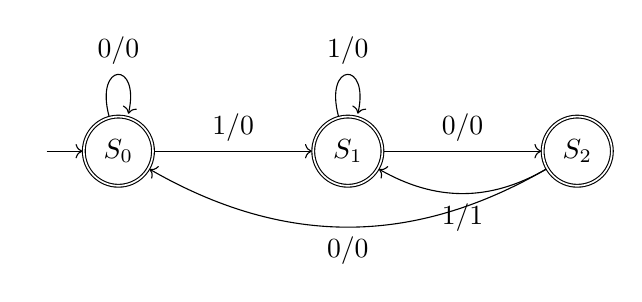
\begin{tikzpicture}[node distance=2cm, initial text={}]
  \node[state, initial, accepting] (S0) {$S_0$};
  \node[state, accepting, right=of S0] (S1) {$S_1$};
  \node[state, accepting, right=of S1] (S2) {$S_2$};
  
  \path[->] (S0) edge[above] node{1/0} (S1)
        (S0) edge[loop above] node{0/0} (S0)
        (S1) edge[above] node{0/0} (S2)
        (S1) edge[loop above] node{1/0} (S1)
        (S2) edge[below,bend left] node{1/1} (S1)
        (S2) edge[below,bend left] node{0/0} (S0);
\end{tikzpicture}
\subsection{\centering Truth Table}
\begin{tabularx}{0.45\textwidth}{
	| >{\centering\arraybackslash}X
	| >{\centering\arraybackslash}X
	| >{\centering\arraybackslash}X
	| >{\centering\arraybackslash}X
    | >{\centering\arraybackslash}X
    | >{\centering\arraybackslash}X
    | >{\centering\arraybackslash}X
	| >{\centering\arraybackslash}X|
	}\hline
	\textbf{$p$}&\textbf{$q$}&\textbf{$x$}&\textbf{$\bar p$}&\textbf{$\bar q$}&\textbf{$y$}&\textbf{$D1$}&\textbf{$D2$}\\
	\hline
	0&0&0&0&0&0&0&0\\
	\hline
	0&0&1&0&1&0&0&1\\
	\hline
    0&1&0&1&0&0&1&0\\
	\hline
	0&1&1&0&1&0&0&1\\
	\hline
	1&0&0&0&0&0&0&0\\
	\hline
	1&0&1&0&1&1&0&1\\
	\hline
	1&1&0&x&x&x&x&x\\
	\hline
	1&1&1&x&x&x&x&x\\
	\hline
\end{tabularx}
\begin{center} 
 Truth table for Boolean function
\end{center}
\subsection{\centering K-Map Implementation of $y$}
\resizebox{0.45\textwidth}{!}{%
	\begin{karnaugh-map}[4][2][1][$qx$][$p$]
		\maxterms{0,1,2,3,4}
		\minterms{5}
        \autoterms[X]
		\implicant{5}{7}
	\end{karnaugh-map}%
}
\begin{center}
Table. 1

herefore, the Boolean function is $y = px$.
\end{center}

\subsection{\centering K-Map Implementation of $D1$}
\resizebox{0.45\textwidth}{!}{%
	\begin{karnaugh-map}[4][2][1][$qx$][$p$]
		\maxterms{0,1,3,4,5}
		\minterms{2}
        \autoterms[X]
		\implicant{2}{6}
	\end{karnaugh-map}%
}
\begin{center}
Table. 2

Therefore, the Boolean function is $D1 = q\bar x$.
\end{center}

\subsection{\centering K-Map Implementation of $D2$}
\resizebox{0.45\textwidth}{!}{%
	\begin{karnaugh-map}[4][2][1][$qx$][$p$]
		\maxterms{0,2,4}
		\minterms{1,3,5}
        \autoterms[X]
		\implicant{1}{7}
	\end{karnaugh-map}%
}
\begin{center}
    Table. 3
    
    Therefore, the Boolean function is $D2 = x$.
\end{center}

	\section{\textbf{Components}}
	\begin{tabularx}{0.45\textwidth}{
			| >{\centering\arraybackslash}X
			| >{\centering\arraybackslash}X
			| >{\centering\arraybackslash}X|
			}
			\hline
			\textbf{Components}&\textbf{Values}&\textbf{Quantity}\\
			\hline
			IOT & & 1\\
			\hline
			Jumper Wires & M-M & 7\\
			\hline
			Breadboard & & 1\\
			\hline
                        LED&&2\\
                        \hline
                        Resistor&220 ohms&2\\
                        \hline
	\end{tabularx}
 
\section{\textbf{Implementation}}
\begin{tabularx}{0.45\textwidth}{
		| >{\centering\arraybackslash}X
		| >{\centering\arraybackslash}X
		| >{\centering\arraybackslash}X|}
\hline
	\textbf{Vaman PIN}&\textbf{INPUT}&\textbf{OUTPUT}\\
	\hline
	2& manual&\\
	\hline
	3&&$LED$\\
	\hline
	13&&$LED$\\
	\hline

\end{tabularx}\\


\textbf{Procedure}
\begin{enumerate}[label={\arabic*}.]
	\item Connect the circuit as per the above table.
	\item Upload the IOT code from  the below link.\\

\begin{tabularx}{0.45\textwidth}{
		| >{\centering\arraybackslash}X|}
	\hline
	https://github.com/SrinathReddyMarri/FWC//
	/blob/master/IOT/main.cpp\\
	\hline

\end{tabularx}\\
	\item Change the values of \textbf{Inputs} in the Hardware and verify the sequence.
\end{enumerate}
\end{document}T
